\documentclass[twoside]{article}

\usepackage{lipsum} % Package to generate dummy text throughout this template

\usepackage[sc]{mathpazo} % Use the Palatino font
\usepackage[T1]{fontenc} % Use 8-bit encoding that has 256 glyphs
\linespread{1.05} % Line spacing - Palatino needs more space between lines
\usepackage{microtype} % Slightly tweak font spacing for aesthetics

\usepackage[hmarginratio=1:1,top=32mm,columnsep=20pt]{geometry} % Document margins
\usepackage{multicol} % Used for the two-column layout of the document
\usepackage[hang, small,labelfont=bf,up,textfont=it,up]{caption} % Custom captions under/above floats in tables or figures
\usepackage{booktabs} % Horizontal rules in tables
\usepackage{float} % Required for tables and figures in the multi-column environment - they need to be placed in specific locations with the [H] (e.g. \begin{table}[H])
\usepackage{hyperref} % For hyperlinks in the PDF

\usepackage{lettrine} % The lettrine is the first enlarged letter at the beginning of the text
\usepackage{paralist} % Used for the compactitem environment which makes bullet points with less space between them

\usepackage{braket}
\usepackage{array}
\usepackage{calc}
\usepackage{graphicx}
\usepackage{listings}
\usepackage{kotex}

\usepackage{amsthm}
\newtheorem{mydef}{Definition}

\lstset{frame=tb,
  language=lisp,
  aboveskip=3mm,
  belowskip=3mm,
  showstringspaces=false,
  columns=flexible,
  basicstyle={\small\ttfamily},
  numbers=none,
  numberstyle=\tiny\color{gray},
  keywordstyle=\color{blue},
  commentstyle=\color{dkgreen},
  stringstyle=\color{mauve},
  breaklines=true,
  breakatwhitespace=true
  tabsize=3}

\lstnewenvironment{Python}
  {\lstset{
  language=Python, 
}}
  {}

\lstnewenvironment{C}
  {\lstset{
  language=C, 
}}
  {}
  
\lstnewenvironment{Java}
  {\lstset{
  language=Java, 
}}
  {}
  
\lstnewenvironment{scheme}
  {\lstset{
  morekeywords={define-type, define, type-case, match}
}}
  {}
  
\lstnewenvironment{expr}
  {\lstset{
	morekeywords={with, deffun, fun}
}}
  {}

\usepackage{color}
\usepackage[table,xcdraw]{xcolor}
\usepackage{adjustbox}


\definecolor{dkgreen}{rgb}{0,0.6,0}
\definecolor{gray}{rgb}{0.5,0.5,0.5}
\definecolor{mauve}{rgb}{0.58,0,0.82}



\hypersetup{%
    pdfborder = {0 0 0}
}



\usepackage{abstract} % Allows abstract customization
\renewcommand{\abstractnamefont}{\normalfont\bfseries} % Set the "Abstract" text to bold
\renewcommand{\abstracttextfont}{\normalfont\small\itshape} % Set the abstract itself to small italic text

\usepackage{titlesec} % Allows customization of titles
%\renewcommand\thesection{\Roman{section}} % Roman numerals for the sections
\renewcommand\thesubsection{\Roman{subsection}} % Roman numerals for subsections
\titleformat{\section}[block]{\large\scshape\centering}{\thesection.}{1em}{} % Change the look of the section titles
\titleformat{\subsection}[block]{\large}{\thesubsection.}{1em}{} % Change the look of the section titles

\usepackage{fancyhdr} % Headers and footers
\pagestyle{fancy} % All pages have headers and footers
\fancyhead{} % Blank out the default header
\fancyfoot{} % Blank out the default footer
\fancyhead[C]{ CS500 Machine Learning and AI} % Custom header text
\fancyfoot[RO,LE]{\thepage} % Custom footer text


%----------------------------------------------------------------------------------------
%	TITLE SECTION
%----------------------------------------------------------------------------------------

\begin{document}
\begin{titlepage}

\newcommand{\HRule}{\rule{\linewidth}{0.5mm}} % Defines a new command for the horizontal lines, change thickness here

\center % Center everything on the page
 
%----------------------------------------------------------------------------------------
%	HEADING SECTIONS
%----------------------------------------------------------------------------------------

\vspace*{3cm}
\textsc{\Large CS500}\\[0.5cm] % Major heading such as course name
\textsc{\large Machine Learning and AI}\\[0.5cm] % Minor heading such as course title

%----------------------------------------------------------------------------------------
%	TITLE SECTION
%----------------------------------------------------------------------------------------

\HRule \\[0.4cm]
{ \huge \bfseries Machine Learning and Artificial Intelligence}\\[0.4cm] % Title of your document
\HRule \\[1.5cm]
 
%----------------------------------------------------------------------------------------
%	AUTHOR SECTION
%----------------------------------------------------------------------------------------

\begin{minipage}{0.4\textwidth}
\begin{flushleft} \large
\emph{Author:}\\
Seungwoo \textsc{Schin} \\% Your name
Chisung \textsc{Song}
\end{flushleft}
\end{minipage}
\begin{minipage}{0.4\textwidth}
\begin{flushright} \large
\emph{Typeset by:} \\
Seungwoo \textsc{Schin} % Supervisor's Name
\end{flushright}
\end{minipage}\\[4cm]

% If you don't want a supervisor, uncomment the two lines below and remove the section above
%\Large \emph{Author:}\\
%John \textsc{Smith}\\[3cm] % Your name

\textsc{ NLP Reading Group, Tensorflow KR}\\[1.5cm] % Name of your university/college

%----------------------------------------------------------------------------------------
%	DATE SECTION
%----------------------------------------------------------------------------------------

%{\large \today}\\[3cm] % Date, change the \today to a set date if you want to be precise
2015 Spring Semester

%----------------------------------------------------------------------------------------
%	LOGO SECTION
%----------------------------------------------------------------------------------------

%\includegraphics{Logo}\\[1cm] % Include a department/university logo - this will require the graphicx package
 
%----------------------------------------------------------------------------------------

%\vfill % Fill the rest of the page with whitespace

\end{titlepage}

% Table of contents 

\tableofcontents
\newpage

\section{Week 2} 

본 주에는 rule-based learning, decision tree, linear regression 기법들에 대하여 다룬다. 

\subsection{Rule-based Learning} 

본 단락에서는 Rule-based 학습 기법에 대해서 다루고자 한다. 먼저 본격적으로 들어가기 전에, 본 단원 전체에서 쓸 용어와 이들의 파이썬 구현을 짚고 넘어가자. 

\begin{itemize} 
\item{Instance $x$ and dataset $D$}

어떤 데이터 하나(datum)를 인스턴스라 하며, 데이터 셋을 $D$라 표기한다. 하나의 데이터는 인스턴스라고 부르며, 인스턴스는 Feature과 Label로 이루어져 있다. 따라서 Feature과 Label의 wrapper 클래스를 아래와 같이 정의하자. 

\begin{Python} 
class Label:
    ''' Wrapper class for label 
    '''
    def __init__(self, label_space):
        self.label_name
        self.label_space = label_space
        
class Feature:
    ''' Wrapper class for feature
    '''
    def __init__(self, feature_name, feature_space):
        self.feature_name = feature_name
        self.feature_space = feature_space
\end{Python}

여기서 각 Feature과 Label이 가지는 attribute중 \_space는 가능한 값을 모두 모아놓은 집합이다. 

위 정의를 이용하면, 각 인스턴스는 결국 위 두 클래스를 이용하여 다음과 같이 정의된다. 데이터셋은 인스턴스 클래스의 집합으로 정의하자. 

\begin{Python} 
class Instance:
    def __init__(self, features, label, is_specificed = True):
        for f in features:
            assert len(f) == 2
            assert isinstance(f[0], Feature)
            assert f[1] in f[0].feature_space
        if is_specified:
            for l in label:
                assert len(l) == 2
                assert isinstance(l[0], Label)
                assert l[1] in l[0].label_space
        else:
            assert isinstance(l, Label)
            
        feature_dict = {}
        for f in feature:
            feature_dict[f[0]] = f[1]
        self.feature_dict = feature_dict
        self.features = features
        self.label = label 

\end{Python}

위 정의에서 어떤 데이터셋의 Feature Space와 Label Space를 다음과 같이 정의할 수 있다. 
\begin{mydef}
\textbf{Feature Space FS}는 인스턴스의 Features들 각각의 feature\_space들의 \href{https://ko.wikipedia.org/wiki/%EA%B3%B1%EC%A7%91%ED%95%A9}{데카르트 곱}으로 정의된다. 
\end{mydef}

\begin{mydef}
\textbf{Label Space FS}는 인스턴스의 Label들 각각의 label\_space들의 \href{https://ko.wikipedia.org/wiki/%EA%B3%B1%EC%A7%91%ED%95%A9}{데카르트 곱}으로 정의된다. 
\end{mydef}

여기서는 굳이 라벨이 하나일 필요는 없게 작성하였으나, 보통은 하나만 쓰는 듯 하다. 
 
\item{Hypothsis $h$ and Hypothesis Space $H$}

$H$는 인스턴스의 Feature space에서 Label Space로 가는 함수의 집합이다. $h$는 $H$의 원소이다. 

\item{Target Function $c$}

Target Function은 우리가 찾고자 하는 함수이며, 임의의 가능한 모든 인스턴스 $x$에 대해서 다음을 만족한다. 여기서 말하는 임의의 인스턴스는 꼭 데이터셋 $D$에 제한되지 않는다. 

\begin{equation} 
c(x.features) = x.labels
\end{equation}

모든 가설은 Target Function과 같은 치역, 공역을 가져야 한다. 

\item{Function Approximation Problem P}

주어진 데이터셋에 대해서 Target Function을 가장 잘 근사하는 함수를 찾는 문제이다. 아래와 같이 파이썬으로 구현될 수 있다. 

\begin{Python} 
class FunctionApproxProblem:
    ''' Fucntion approximation problem. 
    '''
    def __init__(self, F, # feature space
                       L, # Label space
                       D, # Set of instances
                       debug = False):
        for f in F:
            assert isinstance(f, Feature)
        for l in L:
            assert isinstance(l, Label)
        for x in D:
            assert isinstance(x, Instance)
            
        self.F = F
        self.L = L
        self.D = D
\end{Python}
\end{itemize}

본 주에는 일단 classification 문제와 이산적이고 유한한 feature space에 대해서 다룬다고 하자. 그런 경우 $H$가 심각하게 제한되기 때문에 조금 추상적으로 $H$를 모델링하면 편안하게 아래 알고리즘들을 이해할 수 있다.\footnote{ feature space가 Countable Infinite인 경우에도 비슷하게 일반화할 수 있고, 연속적인 경우에는 힘들 것이다.} 

\paragraph{$H$에 대한 고찰} 

어떤 Function Approximation Problem에 대해서, 각 feature의 feature space가 이산적이고 유한하며 feature의 갯수가 유한하고, label도 그러할 때 다음과 같은 그래프 $G(V,E)$를 생각하자. 

\begin{equation} 
V = \{(f_1, f_2, ..., f_i) \in F_1 \times F_2 \times ... \times F_i |f_j \in 2^{F_j}, j<i\}
\end{equation} 

\begin{equation} 
E = \{(v_1, v_2) \in V^2| \exists! j<i, |v_1[j]| = |v_2[j]|+1  \wedge \forall k \neq j, v_1[k] = v_2[k] \}
\end{equation} 
위 그래프는 몇 가지 성질을 가진다. 

\begin{itemize} 
\item $V$와 $H$는 일대일 대응이 가능하다. 다음의 함수를 보면 명백할 것이다. 

\begin{Python} 
def func(v):
    def h(x):
        for idx, f in enumerate(v):
            if not x.features[idx] in f:
                return False
        return True
    return h
\end{Python} 

예를 들어서, $(\phi, \phi, ... , \phi)$의 경우 모든 input에 대해서 False를 리턴할 것이므로, 이론적으로 가장 specific한 함수라 할 수 있다. 사실 공집합을 하나만 가지고 있더라도 언제나 False를 리턴하므로, 일반적으로 생각하는 가장 자연스러운 가설은 노드의 원소 각각이 모두 공집합이 아닐 경우일 것이다. 이러한 vertex들을 여기서는 most specific vertex(MSV)\footnote{말 그대로 여기서의 \textbf{가칭}이므로 다른 곳에서 쓰지 말자.}라고 하자.  $(F_1, F_2, ..., F_i)$는 반대로, 모든 input에 대해서 True를 리턴하므로 가장 general한 함수라고 할 수 있다. 

\item Directed Acyclic Graph(DAG)이다. 이에 따라서 가설공간에서의 partial order를 정의할 수 있다. 이 ordering은 강의노트에서 'more general', 'more specific'과 일치한다. 더 자세히는, $h_1$이 $h_2$보다 일반적이라는 것은 G에서 $h_2$에 대응되는 vertex에서 $h_1$에 대응되는 vertex로 가는 edge가 있음을 의미한다. 이는 위 성질의 설명에서 쓰인 specific/general의 개념과 완전히 일치한다. 

\item V는 $(F_1, F_2, ..., F_i)$에서의 shortest distance로 equivalance relation을 만들 경우 partition되는 set이다. 여기서 거리가 x인 파티션을 $P_d(x)$라고\footnote{이 역시 가칭이다.}  정의하자. 
\end{itemize}

이러한 성질들을 이용하면 아래 find-S 알고리즘과 Candidate Elimination 알고리즘, 더 나아가서는 Decision Tree까지의 알고리즘을 쉽게 이해할 수 있다. 우선 여기서는 Rule-based 학습 방법에 해당하는 find-S 알고리즘과 Candidate Elmination 알고리즘을 알아보고자 한다. 아래에서는 FunctionApproxProblem 클래스의 메소드로 각 알고리즘을 구현하고 위에서 구축한 그래프 기반으로 설명해보고자 한다. 구현은 위 그래프 모델 기반으로 되어있지 않다. 

\paragraph{find-S Algorithm} 

아래는 find-S 알고리즘의 구현이다. 

\begin{Python}         
class FunctionApproxProblem:
    # removed for brevity
    
    def find_S(self, target_label = [True]):
        D = self.D
        F = self.F
        
        # choose most specific function 
        h = {}
        for f in F:
            h[f[0]] = [random.choice(f[0].feature_space)]
        
        for x in D:
            if x.label in target_label:
                for f in x.features:
                    if f[1] in h[f[0]]:
                        pass
                    else:
                        h[f[0]].append(f[1])
        
        # make function 
        def func(x):    
            assert isinstance(x, Instance) and not x.is_specified
            for f in h.keys():
                if not x.feature_dict[f] in h[f]:
                    return False
            return True
        return func # hope Python is functional enought :) 
        
    # removed for brevity
\end{Python} 

원하는 라벨을 가진 인스턴스들의 feature을 고려하여 $H$를 탐색한다. 이 함수는 결국 $H$의 원소 하나를 리턴하게 된다. 위 그래프를 이용한 모델링에서 위 알고리즘을 이해해 보면, MSV 중 하나의 노드에서 출발하여 edge를 따라가는 graph traverse의 종착점을 리턴하는 것으로 이해할 수 있다. 이는 어느 정도 적절한 가설을 찾아주기는 하나, 모든 가능한 가설을 다 포괄하지는 않는다. 따라서 보완하는 알고리즘으로 Version Space를 구축, 이에 따라 구현하는 방법이 있다. 

\paragraph{Version Space Construction \& Candidate Elimination} 

Version Space는 직관적으로 가능한 가설들의 모임으로 볼 수 있다. $H$에 대한 고찰 부분을 참고하여 이해하면, 이는 주어진 데이터셋 D을 잘 설명할 수 있는 파티션의 $P_d(x)$를 고르는 것으로, 모든 데이터셋에 대해서 적절한 $x$의 상한과 하한을 찾는 것이다. 이 때 Version Space는 $\cup_{x \in [l, h]} \{P_d(x)\}$ 로 정의된다. 

구현은 아래와 같다. 

\begin{Python} 
class FunctionApproxProblem:
    
    # removed for brevity
    def _VS_Construction(self, target_labels, debug=False):
    
        # removed for brevity
            
        for f in F:
            s[f] = []
            g[f] = f.feature_space
        
        for x in D:
            if _is_label(x, target_labels):
                # generalize s
                dic = x.feature_dict
                for f in dic.keys():
                    e = dic[f]
                    if e in s[f]:
                        pass
                    else:
                        s[f].append(e)
            else:
                # specialize g
                print(x)
                dic = x.feature_dict
                for f in dic.keys():
                    e = dic[f]
                    g[f].remove(e)
                    break
                    

        s_sum = sum([len(e) for e in s.values()])
        g_sum = sum([len(e) for e in g.values()])
        
        
        for f in product(*[_pow(f.feature_space) for f in F]):
            # removed for brevity
            if s_sum<sum([len(x) for x in f])<g_sum:
                yield _dict2func(dic)
        
    def candidate_elimination(self, target_labels, option='first', debug=False):
        for h in self._VS_Construction(target_labels, debug=debug):
            # removed for brevity
                return h 
\end{Python}


\subsection{Decision Tree} 

위 단락에서는 Rule 기반 학습 방법에 대해서 다뤄 보았다. 본 단락에서는 Decision Tree 기법을 위 기법의 연장선상에서 알아보고 구현해보고자 한다. 기본적으로 모델 세팅은 일치하므로 위 단원에서의 클래스와 표기법을 모두 같이 쓸 것이다. 

\paragraph{Information Gain \& Entropy} 

엔트로피는 통계물리에서 나온 개념으로, 정보이론에서 통계물리에서의 모델을 많이 차용하면서 자연스럽게 같이 사용\footnote{당장 로그가 들어가는 걸 보면 물리학에서의 정의가 연상된다.}되었다. 여기서는 통계물리학적 고찰은 하지 않고, 간단한 예시를 통해 계산법을 살펴보고 이를 이용해 Decision Tree를 구현하는 것만을 살펴보겠다. \footnote{여기서의 예시는 \href{https://ratsgo.github.io/machine\%20learning/2017/03/26/tree/}{Rastro's blog} 에서의 예시를 차용하였다. } 
\begin{figure}
\centering
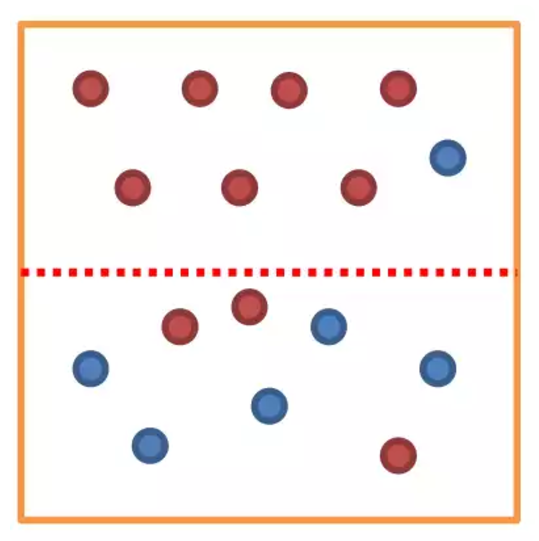
\includegraphics{entropy}
\end{figure}

엔트로피 외에도 이러한 information gain을 계산하는 메트릭은 여러 가지가 있다. 여기서는 간단하게 엔트로피만을 살펴보고자 한다. 

\paragraph{Decision Tree} 

위와 같이 모든 변수에 대해서 최대의 information gain을 얻게 분기하는 경우 decision tree를 얻을 수 있다. 이는 아래와 같이 구현 가능하다. 이러한 Decision Tree의 Ensemble을 이용하여 구현하는 경우 random forest가 된다.  


\subsection{Linear Regression} 

스터디 시간에만 다루면 될 것으로 생각하여 따로 적지 않는다. 



\end{document}



























